\chapter{倫理ある商取引ゲーム}
前章では合理的なプレイヤー達による「商取引ゲーム」において、不正を防止するインセンティブ設計が不可能であることがわかった。
しかしながら、我々は現実の生活の中で商取引で不正に合うことは珍しく、ある程度不正が防止されている。
本章では、この理論と現実の差異は限定合理性にあると仮説立て、
そうした戦略をとるプレイヤーのみで構成されたときに不正を防止することができる「倫理ある商取引ゲーム」をモデリングする。
そして、そのモデルが全ての戦略をとりえるプレイヤーによって構成された「商取引ゲーム」においても、
プレイヤーの構成次第で不正を防止するインセンティブ設計として機能することを示す。

\section{本章における問題提起}
前章では商取引ゲームにおいて必ず不正が防止できるようなインセンティブの設計が不可能であることがわかった。
しかしながら、現実的に私達は商取引で不正行為に遭遇することは稀である。
なぜ先の理論では商取引で不正を防止するインセンティブ設計ができないにも関わらず、
現実の生活の中で我々は商取引を成功させることができているのだろうか。

\section{本章の仮説}
この問いの答えは、限定合理性(Simon 1947\cite{simon 1947})によって戦略の均衡点が変化し、
不正を防止できるインセンティブ設計が可能になっているためだと考えられる。
限定合理性とは、認知能力の限界によって意思決定主体が限られた合理性しか持ち得ていないことである。
各プレイヤーにとっての最適な戦略は他のプレイヤーがとる戦略に依存しているため、
当然、一部のプレイヤーが合理的に戦略を選ばないのであれば最適な戦略の均衡点も変化する。
それによって、全てのプレイヤーが合理的である「商取引ゲーム」においては不可能だった
相手が不正を行う可能性を推定することが可能になり、不正を防止するインセンティブ設計が可能になると予想される。

\section{提案手法}
このような限定合理性を本章では「倫理」と呼ぶ。
提案する「倫理」は、不正行為にあった場合に必ず「失敗」を報告する行動規範とする。
フォーク定理やしっぺ返し戦略が有効であるのと、同様に報復行為である。
この倫理に従うプレイヤーのみで構成される「倫理ある商取引ゲーム」を提案する。
この「倫理」の導入によって、不正が生じた商取引ゲームは必ず失敗が報告されるようになるため、
相手が不正を行う確率の最低値を知ることができ不正を防止するインセンティブ設計が可能になる。

\subsection{倫理ある商取引ゲーム}
「倫理ある商取引ゲーム」においては$buyer$は$seller$が不正を行った場合にかならず「失敗」を報告するため、
ゲーム木は図\ref{ethical-gametree}のようになる.
また、同様に$buyer$が「商取引ゲーム」における戦略$s^{buyer}_2, s^{buyer}_4$を取らないため、
非協力戦略型ゲームの表は表\ref{ethical-gametable}のようになる.

\subsection{誠実な戦略をとった割合と成功が報告される割合の関係}
この「倫理ある商取引ゲーム」においては,商取引の成功率は「商取引システム」に「成功」が報告された割合以上である.
故に、任意のプレイヤー$p$と$q$が過去に「商取引ゲーム」を行った際に、
誠実な戦略($s^{seller}_1$もしくは$s^{buyer}_1$)をとってきた割合$HonestStrategyRate(p, q)$と、
成功が報告された割合$ReportedSuccessRate(p, q)$について、次の関係がいえる。

\begin{equation}
  HonestStrategyRate(p, q) \geq ReportedSuccessRate(p, q)
\end{equation}

\subsection{不正が抑制される戦略組と期待利得の不等式}
「倫理ある商取引ゲーム」において、不正を防止するためには、
$seller$と$buyer$の戦略組を$(s^{seller}_1, s^{buyer}_1)$に帰着させる必要がある。.
そのためには$seller$が戦略$s^{seller}_1$をとった場合の期待利得$E(r|s^{seller}_1)$が
戦略$s^{seller}_2$をとった場合の期待利得$E(r|s^{seller}_2)$より大きく,
$buyer$が戦略$s^{buyer}_1$をとった場合の期待利得$E(r|s^{buyer}_1)$が
戦略$s^{buyer}_3$をとった場合の期待利得$E(r|s^{buyer}_3)$より大きくならなければならない.
つまりは,$E(r|s^{seller}_1) > E(r|s^{seller}_2)$かつ$E(r|s^{buyer}_1) > E(r|s^{buyer}_3)$を満たす
$(r^{seller}_{success}, r^{seller}_{failure}, r^{buyer}_{success}, r^{buyer}_{failure})$の組を
「商取引システム」から決定できる必要がある.

\subsection{$ seller $と$ buyer $の期待利得}

$ seller $と$ buyer $の各戦略の利得の期待値は以下のように表せる.\\


$ E(R|s^{seller}_1) = p^{buyer}_1 (r^{seller}_{success} + \epsilon^{seller}) + p^{buyer}_3 (r^{seller}_{failure} + \lambda^{seller}) $ \\

$ E(R|s^{seller}_2) = p^{buyer}_1 (goods + r^{seller}_{failure} + \lambda^{seller}) + p^{buyer}_3 (goods + r^{seller}_{failure} + \lambda^{seller}) $ \\

$ = goods + r^{seller}_{failure} + \lambda^{seller} $ \\

$ \because p^{buyer}_1 + p^{buyer}_3 = 1 $(「倫理ある商取引ゲーム」において、$ p^{buyer}_2 $と$ p^{buyer}_4 $は0であるため) \\

$ E(R|s^{buyer}_1) = p^{seller}_1 (goods + r^{buyer}_{success} + \epsilon^{buyer}) + p^{seller}_2 (r^{buyer}_{failure} + \lambda^{buyer}) $ \\

$ E(R|s^{buyer}_3) = p^{seller}_1(goods+r^{buyer}_{failure} + \lambda^{buyer}) + p^{seller}_2 (r^{buyer}_{failure} + \lambda^{buyer}) $ \\

$ = p^{seller}_1 goods + r^{buyer}_{failure} + \lambda^{buyer} $ \\

$ \because p^{seller}_1 + p^{seller}_2 = 1 $ \\


\subsection{$ seller $が誠実な戦略をとる条件}

$ E(R|s^{seller}_1) > E(R|s^{seller}_2) $ \\

$ \therefore p^{buyer}_1 (r^{seller}_{success} + \epsilon) + p^{buyer}_2 (r^{seller}_{failure} + \lambda) > goods + r^{seller}_{failure} + \lambda $ \\

$ \therefore p^{buyer}_1(r^{seller}_{success} + \epsilon) - p^{buyer}_1(r^{seller}_{failure} + \lambda) > goods $ \\

$ \therefore p^{buyer}_1(r^{seller}_{success} - r^{seller}_{failure} + \epsilon - \lambda) > goods $ \\

仮定より,$ \epsilon > \lambda $のため,
$ p^{buyer}_1 (r^{seller}_{success} - r^{seller}_{failure}) \geq goods $を満たせばよい.

$ 0 < p^{buyer}_1 $を仮定するならば,
$ r^{seller}_{success} - r^{seller}_{failure} \geq \frac{goods}{p^{buyer}_1} $


\subsection{$ buyer $が誠実な戦略をとる条件}

$ E(R|s^{buyer}_1) > E(R|s^{buyer}_3) $ \\

$ \therefore p^{seller}_1 (goods + r^{buyer}_{success}) + p^{seller}_2 r^{buyer}_{failure} > p^{seller}_1(goods+r^{buyer}_{failure}) + p^{seller}_2 r^{buyer}_{failure} $ \\

$ \therefore p^{seller}_1(r^{buyer}_{success} - r^{buyer}_{failure}) > 0 $ \\

$ 0 < p^{seller}_1 $を仮定するならば, \\

$ r^{buyer}_{success} - r^{buyer}_{failure} > 0 $ \\

上記をまとめると,$ 0<p^{buyer}_1 $かつ $ 0 < p^{seller}_{1} $を仮定した上で,\\

$ r^{seller}_{success} - r^{seller}_{failure} \geq \frac{goods}{p^{buyer}_1} $かつ$ r^{buyer}_{success} - r^{buyer}_{failure} > 0 $ \\

を満たせば,「倫理ある商取引ゲーム」で不正を防止することができる.


\subsection{信頼度 $ p^{player} $}

ここで,任意の$ player $が誠実な戦略($ p^{seller}_1, p^{buyer}_1 $のいづれか)をとる主観確率を$ p^{player}_1 $とすると,
$ p^{player}_1 $は各プレイヤーに対して誠実な戦略をとった割合$ HonestyStrategyRate(player, opportunity) $と任意の重み$ w^{player} $を用いて次のように表せる. \\

\begin{equation}
  p^{player}_1 \equiv \sum^{players}_{opp} w^{opp} HonestyStrategyRate(player, opp)
\end{equation}

\subsection{最低信頼度 $ T^{player} $}

しかし、「商取引システム」からは$ HonestyStrategyRate(player, opportunity) $は未知のため,
信頼度$ p^{player}_1 $を求めることができない.
そこで$ HonestyStrategyRate $の代わりに$ ReportedSuccessRate $を用い、
信頼度$ p^{player} $を計算するのと同じ重み$ w^{player} $の荷重総和をとったものを、
最低信頼度$ T^{player} $と定義する. \\

\begin{equation}
  T^{player} \equiv \sum^{players}_{opp} {w}^{opp} ReportedSuccessRate(player, opp)
\end{equation}

\subsection{最低信頼度を用いた条件}
ここで$ HonestyStrategyRate \geq ReportedSuccessRate $であるため,$ p^{player}_1 \geq T^{player} $がいえる.

ゆえに, \\

\begin{equation}
  r^{seller}_{success} - r^{seller}_{failure}  \geq \frac{goods}{T^{buyer}} \geq \frac{goods}{p^{buyer}_1}
\end{equation}

となる.

つまり、$ 0<p^{buyer}_1 $かつ $ 0 < p^{seller}_{1} $を仮定した上で,\\

\begin{equation}
  r^{seller}_{success} - r^{seller}_{failure} \geq \frac{goods}{T^{buyer}} かつ r^{buyer}_{success} - r^{buyer}_{failure} > 0
\end{equation}

を満たす$ (r^{seller}_{success}, r^{seller}_{failure}, r^{buyer}_{success}, r^{buyer}_{failure}) $の組を「商取引システム」から決定できれば、
「倫理ある商取引ゲーム」において不正を防止することができる。


\section{実験方法}
個々で実装の詳細にも少し触れる。

\section{評価}

\section{結論}


\clearpage
\begin{figure*}
  \centering
  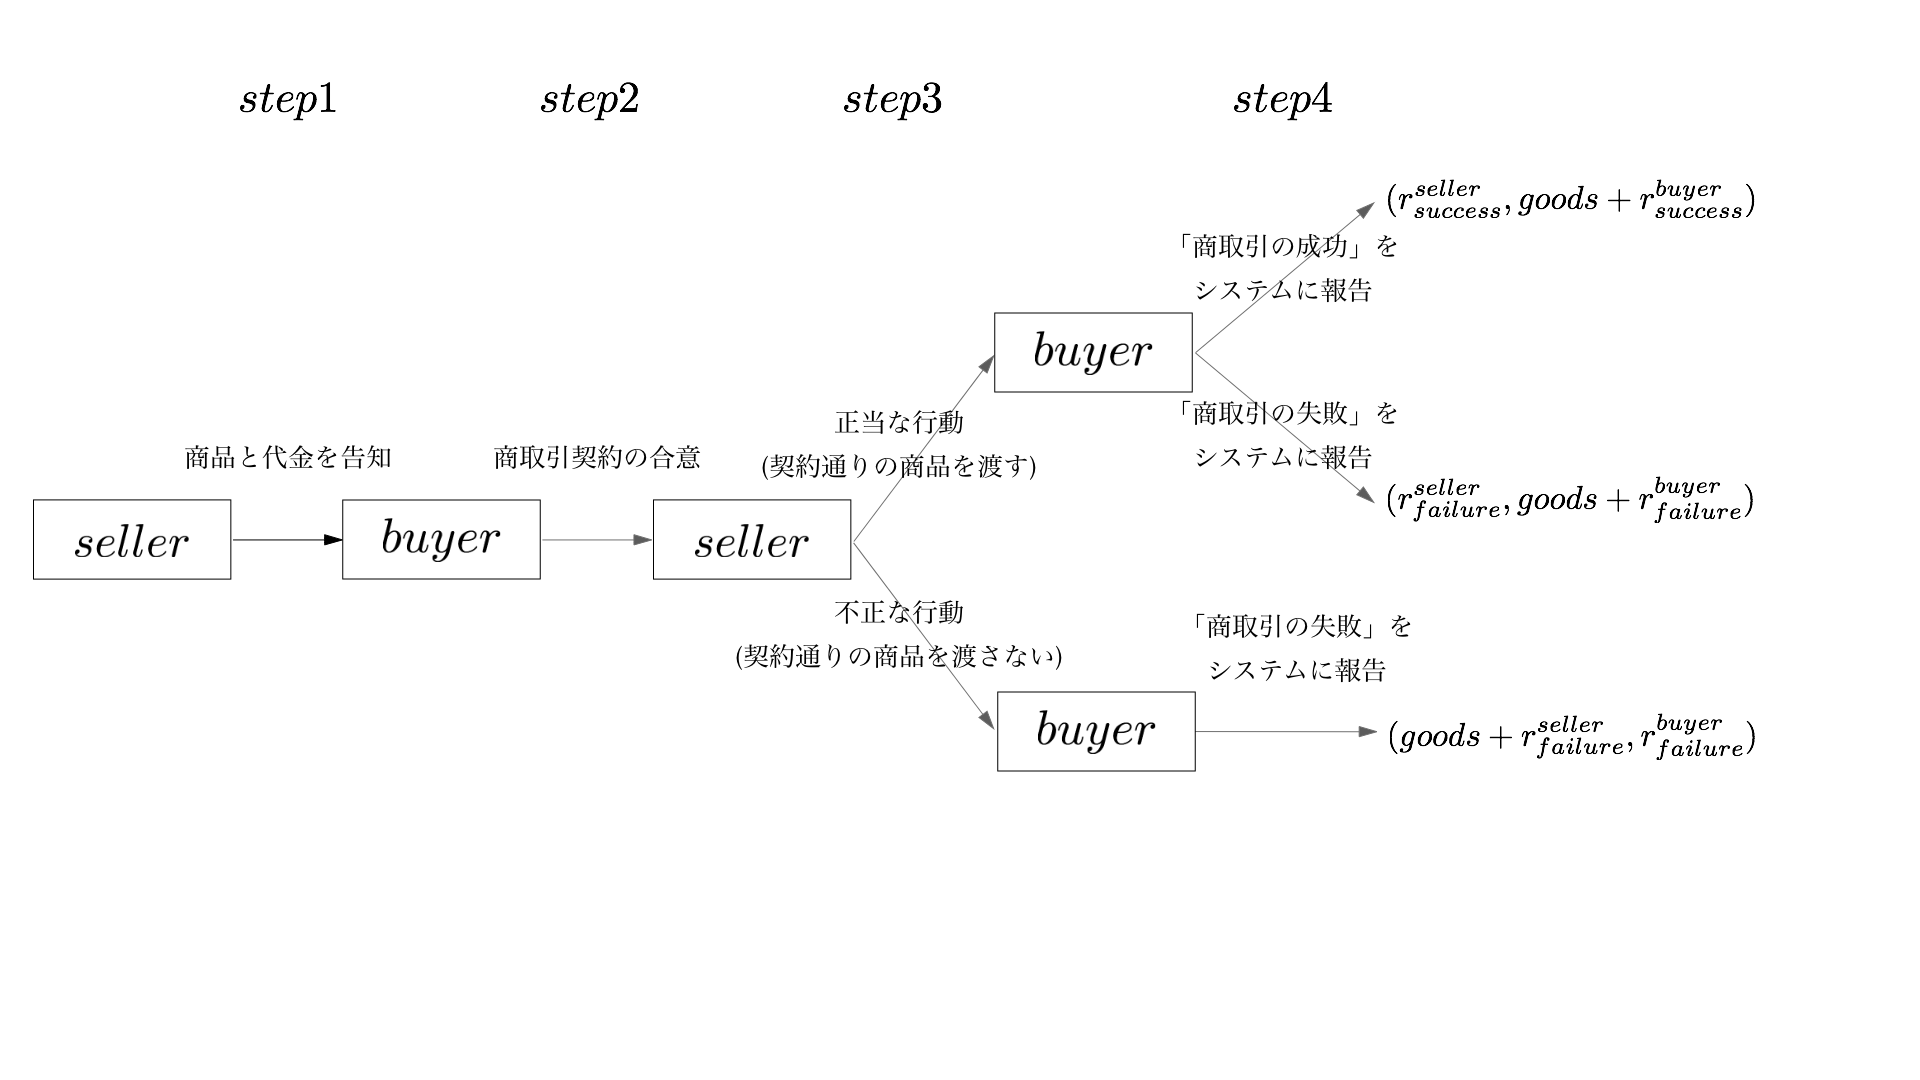
\includegraphics[width=1\linewidth]{./06_ethical-commerce-game/ethical-gametree.png}
  \caption{「倫理ある商取引ゲーム」のゲーム木}
  \label{ethical-gametree}
\end{figure*}

\subsection{非協力戦略型ゲーム}
\newcommand{\successseller}{
  \begin{tabular}{c}
    $(r^{seller}_{success},$\\
    $goods+r^{buyer}_{success})$
  \end{tabular}
}
\newcommand{\successbuyer}{
  \begin{tabular}{c}
    $(goods+r^{seller}_{success},$\\
    $r^{buyer}_{success})$
  \end{tabular}
}
\newcommand{\fseller}{
  \begin{tabular}{c}
    $(r^{seller}_{failure},$\\
    $goods+r^{buyer}_{failure})$
  \end{tabular}
}
\newcommand{\fbuyer}{
  \begin{tabular}{c}
    $(goods+r^{seller}_{failure},$\\
    $r^{buyer}_{failure})$
  \end{tabular}
}

\begin{table*}
  \centering
  \begin{tabular}{|l|l|l|l|}
    \hline
    \multicolumn{2}{|l|}{\multirow{2}{*}{}} & \multicolumn{2}{l|}{$buyer$} \\ \cline{3-4}
    \multicolumn{2}{|l|}{}                  &$s^{buyer}_1$&$s^{buyer}_3$\\ \hline
    \multirow{2}{*}{$seller$}
    &$s^{seller}_1$&\successseller&\fseller\\ \cline{2-4}
    &$s^{seller}_2$&\fbuyer&\fbuyer\\ \hline
  \end{tabular}
  \caption{非協力戦略型ゲームとして表した「倫理ある商取引ゲーム」の利得表}
  \label{ethical-gametable}
\end{table*}

% \subsection{自己信頼}
ここで$ HonestStrategyRate(player, player) $と$ ReportedSuccessRate(player, player) $は1とする.これは$ player $が$ player $自身と行う商取引は必ず成功するためである.

\subsection{将来期待利得}
通常の「商取引ゲーム」においては誠実な戦略を取ってきた割合と報告された商取引ゲームの成功率の間の関係性はわからないため,繰り返しゲームと考えても次のゲームへ引き継げる情報がなかったため将来期待利得を考慮しなかったが,「倫理ある商取引ゲーム」においては先に述べた関係式が得られるため,将来期待利得を考慮する必要がある.商取引で「成功」が報告された場合の$ seller $と$ buyer $の将来期待利得を$ \epsilon^{seller}, \epsilon^{seller} $とし,「失敗」が報告された場合の将来的な期待利得を$ \lambda^{seller}, \lambda^{buyer} $とおくと,「倫理ある商取引ゲーム」のゲーム木と非協力戦略型ゲームの表は次のように書き換えられる.
また,本稿では,これらについて$ \epsilon^{player} > \lambda^{player} $と仮定する.


% 倫理ある商取引ゲーム
% \section{倫理ある商取引システムの詳細}
「倫理ある商取引ゲーム」においては,最低信頼度$ T^{player} $を用いた上記の条件式を満たせば,不正を防止することが可能になる.ただ,上記の条件のみでは「商取引システム」から保有通貨の変化量の組$ (r^{seller}_{success}, r^{seller}_{failure}, r^{buyer}_{success}, r^{buyer}_{failure}) $を一意に決定できないので,いくつかの条件を追加する.


\subsection{取引成功前後の残高の変化}
商取引成功前後では$ buyer $は商品$ goods $の価格$ price $だけ残高が減り$ seller $は$ price $だけ残高が増えるものとする.そのため商取引前後では$ seller $と$ buyer $の残高の合計は変化しない.ここから,$ r^{seller}_{success} $と$ r^{buyer}_{success} $は以下のように記せる.

$ r^{seller}_{success} = price $
$ r^{buyer}_{success} = -price $
$ r^{seller}_{success} + r^{buyer}_{succcess} = 0 $

\subsection{エスクロー係数 E}
まずは「失敗」が報告された時に$ seller $と$ buyer $から失われる通貨の量の合計を$ EscrowCost $とおいて考え,同時に商品価格$ price $にエスクロー係数$ E $を掛けたものとする.(ここで$ price $は$ goods $の価格である)

$ EscrowCost \equiv (r^{buyer}_{success} - r^{buyer}_{failure}) + (r^{seller}_{success} - r^{seller}_{failure}) $
$ = E \cdot price $

\subsection{負担比率}
ここで問題となるのは$ EscrowCost $を求めるための$ seller $と$ buyer $の負担比率をどのようにして決定するかである.本稿では最低信頼度$ T^{player} $を用いてこの負担比率を決定することとする.

$ (r^{buyer}_{success} - r^{buyer}_{failure}):(r^{seller}_{success} - r^{seller}_{failure}) = w(T^{buyer}):w(T^{seller}) $

ここで最低信頼度が高い$ player $の方が負担比率が小さくなるように責任比重関数$ w(x) $は値域$ 0 \leq  x \leq 1 $において$ w'(x)>0 $を満たすものとする.

\subsection{責任比重関数$ w(x) $}
本稿では負担比重関数は恒等写像$ w(x)=x $とする.

\subsection{ReputationWeights}
最低信頼度$ T^{player} $を求めるにあたって$ r.w.^{opportunity} $を決定する必要がある.$ r.w.^{opportunity} $は誠実さ$ T^{player}_1 $を求める際に$ ReportedSuccessRate(player, opportunity) $に係る任意の重みである.これはつまり任意の$ player $が誠実な戦略をとる主観的確率を考える際に,$ player $と$ opportunity $の間であった過去の商取引での報告された成功率をどの程度信じるかである.仮に$ player $と$ opportunity $の間で信頼関係があれば$ ReportedSuccessRate $は$ 1 $になる.なので「商取引システム」の参加者数$ n $が特定できる場合は$ \frac{1}{n} $が妥当だろう.逆に不特定多数であり,同一の意志によって複数のプレイヤーが動いている場合は,保有している通貨量$ b^{opportunity} $の全体の通貨の総量に占める割合が良いだろう.

$ r.w.^{opportunity} \equiv \frac{b^{opportunity}}{\sum^{players}_{i}b^{i}} $


\subsection{EscrowCostの分配}
「失敗」が報告されたときに失われる$ EscrowCost $は消滅するのではなく参加者に分配する.これは全体の通貨量の減少によって通貨の価値が上がって商品価格が下がるという経済原理が生じ,インセンティブ設計が複雑化するのを防ぐためである.そこで$ EscrowCost $として失われた通貨は任意の重み$ e.w.^{player} (\sum^{players}_{player}e.w.^{player} = 1) $を用いて分配し「商取引ゲーム」の前後で全体の通貨量を等しくする.

\subsection{EscrowWeights}
EscrowCostの分配に関しては「商取引システム」に参加している各プレイヤーの通貨の保有率に応じて分配する.$ seller $と$ buyer $を含んでいるのは,仮に$ seller $と$ buyer $以外のすべてのプレイヤーで分配した場合,$ seller $もしくは$ buyer $は結託する別のプレイヤーに保有する通貨の一部を一時的に預けることで,その分だけ$ EscrowCost $の負担を軽減することが可能になるためである.そこで本稿では任意の重み$ e.w.^{player} $を以下のように定義する.

$ e.w.^{player} \equiv \frac{b^{player}}{\sum^{players}_{escrow}b^{escrow}} $

\subsection{謎の条件}
$ \frac{w(T^{buyer}_1)E \cdot price}{w(T^{buyer}_1) + w(T^{seller}_1)} \geq \frac{price}{T^{buyer}} \geq \frac{goods}{p^{buyer}_1} $

上記の条件式から$ \frac{price}{ T^{buyer} } $でうまくいくはずだったが何故かうまく行かず,$ \frac{price}{ \min(T^{buyer}, T^{seller})} $をもちいたらうまくいったのでこちらを採用することとした.$ p^{buyer} $と$ P^{player}_1 $の関係性に問題があるためだと思われる.

$ \frac{w(T^{buyer}_1)E \cdot price}{w(T^{buyer}_1) + w(T^{seller}_1)} \geq \frac{price}{ \min(T^{buyer}, T^{seller})} $


\subsection{残高の変化量の組$ (r^{seller}_{success}, r^{seller}_{failure}, r^{buyer}_{success}, r^{buyer}_{failure}) $}
上記の条件群を用いて残高の変化量の組$ (r^{seller}_{success}, r^{seller}_{failure}, r^{buyer}_{success}, r^{buyer}_{failure}) $を決定する.


$ r^{seller}_{success}+r^{buyer}_{success} = 0 $

$ r^{seller}_{failure}+r^{buyer}_{failure} = -E \cdot price $

$ r^{seller}_{success} - r^{seller}_{failure} = \frac{w(T^{buyer}_1)E \cdot price}{w(T^{buyer}_1) + w(T^{seller}_1)} \geq \frac{price}{T^{buyer}} $

$ r^{buyer}_{success} - r^{buyer}_{failure} = \frac{w(T^{seller}_1)E \cdot price}{w(T^{buyer}_1) + w(T^{seller}_1)} \geq 0 $

$ \frac{w(T^{buyer})E \cdot price}{w(T^{buyer}) + w(T^{seller})} = \frac{price}{\min(T^{buyer}, T^{seller})} $

$ E $ = $ \frac{w(T^{buyer})+w(T^{seller})}{w(T^{buyer}) \cdot \min(T^{buyer}, T^{seller})} $

$ r^{seller}_{success}-r^{seller}_{failure} = \frac{price}{min(T^{buyer}, T^{seller})} $

$ r^{buyer}_{success} - r^{buyer}_{failure} = \frac{w(T^{seller}) \cdot price}{w(T^{buyer}) \cdot \min(T^{buyer}, T^{seller})} $


$ r^{seller}_{success} = price $
$ r^{buyer}_{success} = -price $
$ r^{seller}_{failure} = price \cdot (1 - \frac{1}{min(T^{buyer}, T^{seller})}) $
$ r^{buyer}_{failure} = - price \cdot (\frac{T^{seller}}{T^{buyer} \cdot \min(T^{buyer}, T^{seller})} + 1) $

% \section{実験方法}
提案手法を用いることで不正が防止されるかどうかを検証するためにコンピューターシミュレーションを用いた実験を行う.この実験では$ (s^{seller_1}, s^{seller}_2) $と$ (s^{buyer}_1, s^{buyer}_2, s^{buyer}_3, s^{buyer}_4) $から任意の戦略組をもつエージェント(全8通り)を10機用意して下記の試行を繰り返す.試行ごとに過去100回分の「真の商取引の成功率(TrueSuccessRate)」と「商取引システム」に「報告された成功率(ReportedSuccessRate)」を記録する.

①10機のエージェントからランダムに$ seller $と$ buyer $を決定し「商取引ゲーム」を行う.
②残高の変化量の組$ (r^{seller}_{success}, r^{buyer}_{success}, r^{seller}_{failure}, r^{buyer}_{failure}) $を算出し,「失敗」が報告された場合に$ seller $と$ buyer $の残高が0未満にならないかを判定する.ここで0未満になる場合は再度,①からやり直し,100回連続で
③$ seller $と$ buyer $のエージェントは戦略から「商取引システム」に報告される結果を決定する.
④「商取引システム」は報告された結果に応じてすべてのエージェントの残高を操作する.
⑤試行回数が10000回になるまで①から④を繰り返す.

\subsection{「 倫理ある商取引ゲーム」での実験}
「倫理ある商取引ゲーム」では$ seller $と$ buyer $がとりえる戦略は$ (s^{seller_1}, s^{seller}_2) $と$ (s^{buyer}_1, s^{buyer}_3 $のみであるため,これらを組み合わせた4パターンのエージェントを全体で10機用意して実験を行う.この10機の4パターンでの構成は268通りあるので,その全て場合で1回づつ実験を行う.

\subsection{「商取引ゲーム」での実験}
「倫理ある商取引ゲーム」では$ seller $と$ buyer $がすべての戦略をとりえるため,8パターンのエージェントを全体で10機用意して実験を行う.この10機の4パターンでの構成は19960通りあるので,モンテカルロ法を用いてランダムに重複ありの1000パターンの構成を生成し実験を行う.

% \section{評価}

\begin{figure}[h]
  \begin{tabular}{cc}
    %---- 最初の図 ---------------------------
    \begin{minipage}[t]{1\hsize}
      \centering
      % \includegraphics[keepaspectratio, width=1\linewidth]{ethical-aggregate.png}
      \caption{「倫理ある商取引ゲーム」}
      \label{ethical-experiment-aggregate}
    \end{minipage} \\
    %---- 2番目の図 --------------------------
    \begin{minipage}[t]{1\hsize}
      \centering
      % \includegraphics[keepaspectratio, width=1\linewidth]{no-ethical-aggregate.png}
      \caption{「商取引ゲーム」}
      \label{non-ethical-experiment-aggregate}
    \end{minipage}
    % ---- 図はここまで ----------------------
  \end{tabular}
\end{figure}

\subsection{「倫理ある商取引ゲーム」での評価}
「倫理ある商取引ゲーム」における286回の実験データを誠実なエージェントの数ごとに集計し,「商取引ゲーム」を10000万回を繰り返したときの真の成功率の平均をプロットしたのがFigure\ref{ethical-experiment-aggregate}である.誠実なエージェントが3機以下の場合は真の商取引の成功率の平均はいずれも0\%であったが,5機以上の場合はいずれも100\%に収束していた.

\subsection{「商取引ゲーム」での評価}
同様に,通常の「商取引ゲーム」における1000件の実験データを誠実なエージェントの数ごとに集計し,「商取引ゲーム」を10000万回を繰り返したときの真の成功率の平均をプロットしたのがFigure\ref{non-ethical-experiment-aggregate}である.こちらも誠実なエージェントが5機以上の場合は真の商取引の成功率の平均はいづれも99\%を超えていた.また,「倫理ある商取引ゲーム」での実験に比べて4機の場合に比べてこちらの方が真の商取引の成功率の平均は高かく,3機以下の場合でも完全に0\%にはならなかった.

% \section{考察}
「倫理ある商取引ゲーム」において誠実なエージェントが1体以下の場合,どの2体のエージェントで「商取引ゲーム」を行っても商取引は失敗する.そのため誠実なエージェントが1体以下の場合に商取引の成功率が0\%になるのは納得である.しかし,今回の実験では2体もしくは3体の場合でも真の商取引の成功率の平均が0\%になっている.この点は疑問である.また,今回のインセンティブ設計のアルゴリズムは「倫理ある商取引ゲーム」を前提としているにも関わらず,通常の「商取引ゲーム」の方が誠実なエージェントが4体のときの真の商取引の成功率の平均値が高いのは不可解である.これらの原因としては,確率的な試行であるにも関わらず「倫理ある商取引ゲーム」においては286パターンのエージェントの構成で1回づつしかサンプリングを行っていないことや,エージェントの構成が19960パターン考えられる通常の「商取引ゲーム」で1000回しか試行をしていないことなどが原因として考えられる.また,最低信頼度$T^{player}$と誠実さ$P^{player}_1$の関係性が$p^{buyer}_1$との関係性とすり替わっていることも原因として考えられる.実験方法やインセンティブ設計を修正する必要があると思われる.現状の結果から唯一いえることがあるとすれば,誠実なエージェントの割合が一定を超えると「商取引ゲーム」の不正行為が防止できるということである.
